% !TEX root = ../../thesis.tex


\cleartoleftpage
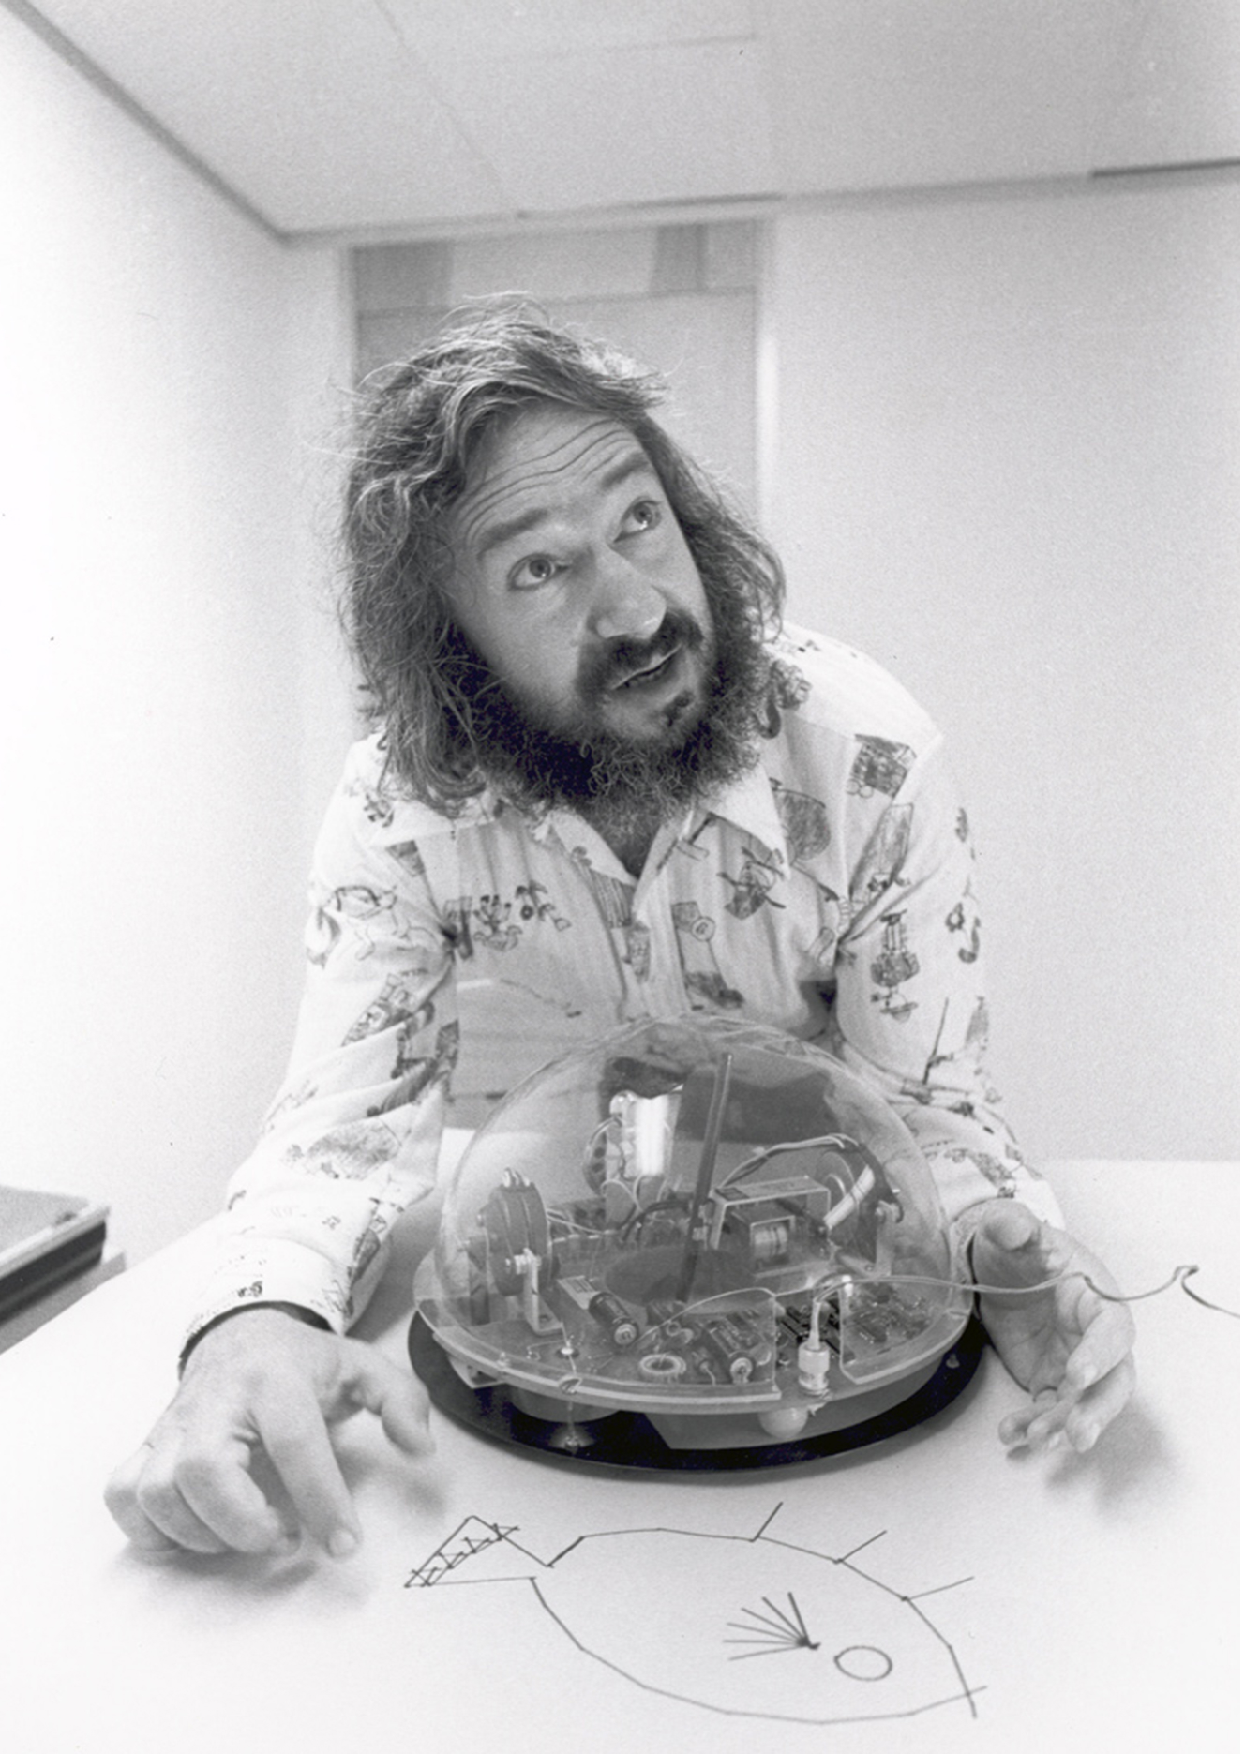
\includepdf{../media/chapter_illustration/seymour-papert.pdf}

\chapter{Education} % (fold)
\cleanchapterquote{New technologies help students navigate the creative thinking spiral.}{Mitchel Resnick}


\section{Introduction} % (fold)

In our modern societies, in particular in France, education is a top priority and concern for government and people. Thus education is central and has to be adapted and relevant following societal evolution. In particular, new technologies have a deep impact on our societies and raised legitimate question and worry~\cite{plester2008txt}. Also, they can become great vectors to make the educational system more efficient and fair.


\textbf{1- Improve education accessibility and dissemination:}

Knowledge is a humanity wealth and thanks to the very large democratization of Internet, anyone with a connection can now, access the whole humanity knowledge in just a couple of second. The most famous example is certainly Wikipedia\footnote{\url{http://www.wikipedia.org/}}, a community encyclopedia with a non-stop growing content both in term of quantity and quality. With such tool, anyone can access instantly to anything one wants to know, from the history of French "crêpes"\footnote{\url{http://en.wikipedia.org/wiki/Crêpe}} to the explanation of the most famous quantum mechanics principles\footnote{\url{http://en.wikipedia.org/wiki/Schrödinger_equation}}.

In addition to global encyclopedia referencing -almost- all the humanity knowledge, the use of Internet is also changing the way we learn. Indeed, there is more and more website designed to share free online courses. One of the first success is the Khan Academy.
The Khan Academy\footnote{\url{https://www.khanacademy.org/}} is an educational website founded by Salman Khan which discusses, along about 2.400 videos, principles of math, science, and economics.  It's aimed at helping people master the basics, the humble bread-and-butter equations they encounter in elementary and high school. In addition to the video, the website offers software that tracks evolution of learning, generates practice problems and use gamefication to reward performance.
Complementary to Khan's site which is ruthlessly practical and oriented to the master of basics~\cite{thompson2011khan}, the most famous Universities are beginning to freely diffuse theirs advanced courses other Internet, we can cite as example the MIT open course ware (OCW)\footnote{\url{http://ocw.mit.edu/}} or the open Yale courses\footnote{\url{http://oyc.yale.edu/}}.

Finally, a current growing buzz concerns the creation of massive open online courses (MOOC)~\cite{mackness2010ideals}.

\begin{quotation}
    A MOOC integrates the connectivity of social networking, the facilitation of an acknowledged expert in a field of study, and a collection of freely accessible online resources. Perhaps most importantly, however, a MOOC builds on the active engagement of several hundred to several thousand “students” who self-organize their participation according to learning goals, prior knowledge and skills, and common interests.[...]A MOOC generally carries no fees, no prerequisites other than Internet access and interest, no predefined expectations for participation, and no formal accreditation.
    \signed{Alexander McAuley and al. The MOOC model for digital practice.~\cite{mcauley2010mooc}}
\end{quotation}

MOOCs are a recent development in distance education which began to emerge in 2012~\cite{pappano2012year}. In France, a first step was done in the end of October 2013 with the creation of the website France Université Numérique\footnote{\url{http://www.france-universite-numerique.fr/}}, trying to promote the development of MOOC teaching in France.


\textbf{2- Teaching people being comfortable with and aware of the digital world}

\textbf{[help] du contenu pour dire qu'apprendre le "numérique" c'est important ?}

\begin{quotation}

    It has become common place to refer to young people as “digital natives,” because of their apparent fluency with digital technologies. And, indeed, many young people are very comfortable sending text messages, playing online games, and browsing the web. But does that really make them fluent with new technologies? Although young people interact with digital media all of the time, few of them can create their own games, animations, or simulations. It’s as if they can "read" but not "write".
    \signed{Mitchel Resnick and al. Scratch: Programming for Everyone~\cite{resnick2009scratch}}

\end{quotation}

To introduce computer concepts to children, MIT Media Lab developed Scratch~\cite{resnick2009scratch} forked by Berkeley into Snap an extended reimplementation of Scratch which makes it suitable for a serious introduction to computer science for high school or college students. With its block interface, it allows to code by combining block such as Lego one.

\begin{quotation}
    Digital fluency requires not just the ability to chat, browse, and interact, but also the ability to design, create, and invent with new media~\cite{resnick2008sowing}. To do that, you need to learn some type of programming. The ability to program offers many important benefits: it greatly expands the range of what you can create (and how you can express yourself) with the computer, while also expanding the range of what you can learn. In particular, programming supports the development of “computational thinking,” helping you learn important problem-solving and design strategies (such as modularization and iterative design) that carry over to non-programming domains. And since programming involves the creation of external representations of your problem-solving processes, programming provides you with opportunities to reflect on your own thinking and even to think about thinking itself~\cite{disessa2001changing}

    \signed{Mitchel Resnick and al. Scratch: Programming for Everyone~\cite{resnick2009scratch}}

\end{quotation}


\textbf{3- Using robots as new pedagogical tools}

Robots have a great potential of becoming an ideal tools for teaching a wide range of engineering disciplines. Indeed, robots are intrinsically multidisciplinary objects embedding elements from diverse fields among them computer science, mechanics, electronics or signal processing. Also they are a great motivation tool because they permit instantly applications in the real world giving meaningful context favorable for constructivist teaching~\cite{palincsar1998social} \cite{papert1991situating}. There is already several great success examples such as the e-puck robot~\cite{mondada2009puck} which specifically targets engineering education at university level or Thymio II adapted for teaching robotic and computer science in primary education~\cite{riedo2012two}~\cite{riedo2013thymio}.
% Also the now famous Arduino boards~\cite{mellis2007arduino} and Fablabs


\section{Education and the Poppy project} % (fold)

The Poppy platform was initially designed for research purposes and even more specifically for studying biped locomotion and human-robot interaction. However, its conception has been made with open science goals, both to share our research and create tools for researchers. As we are convinced in the need of multidisciplinary contributions in order to improve the state of the art in the robotics field, we decided right from the beginning to use and create modern and easy-to-use tools. This choice as strongly impacted the way we designed our platform. Indeed being simple to use, easily reproducible and hackable, modular, 3Dprintable and as plug'n'play as possible lead to the development of hardware (Poppy) and software (pypot) tools which can be also used by non-expert people.

Thus Poppy meets a growing societal need: education and training in technologies combining computer science, electronics and mechanics, as well as a training tool to the emergent revolutionary 3D printing process. Since October 2013 (open source release), we have been contacted by several Fablabs, universities, engineering schools and even high schools. We had the opportunity to have meetings with some educational teams and it appears they were looking for new motivating tools for group projects.

In this context, the Poppy platform appears well suited. Indeed, it integrates advanced and yet easily accessible techniques (3D printing, Arduino, Python) in an embodiment that motivates students and the wider public. With its openness, its design and its rather low-cost, Poppy is highly hackable and provides an unique context for experimentation and learning of these technologies in a Do-It-Yourself (DIY) approach.

Several experiences with Poppy in secondary, high schools, science museums and Fablabs in France and abroad are already underway and will be discussed in the incoming sections.


\section{scientific mediation} % (fold)
\label{sec:poppy_universience}

On march 22th \& 23th 2014, UniverSciences\footnote{Paris museum of sciences and technologies} organized a hackathon for the general public around the assembly of a Poppy robot (see \figurename~\ref{fig:universience_hackathon_orga}). It involved 21 robotic enthusiasts (aged from 23 to 46) with various backgrounds (informatics, electronics, physics, sociology, mechanics, architecture).

\begin{figure}[t]
\centering
    \subfloat[][Introduction]{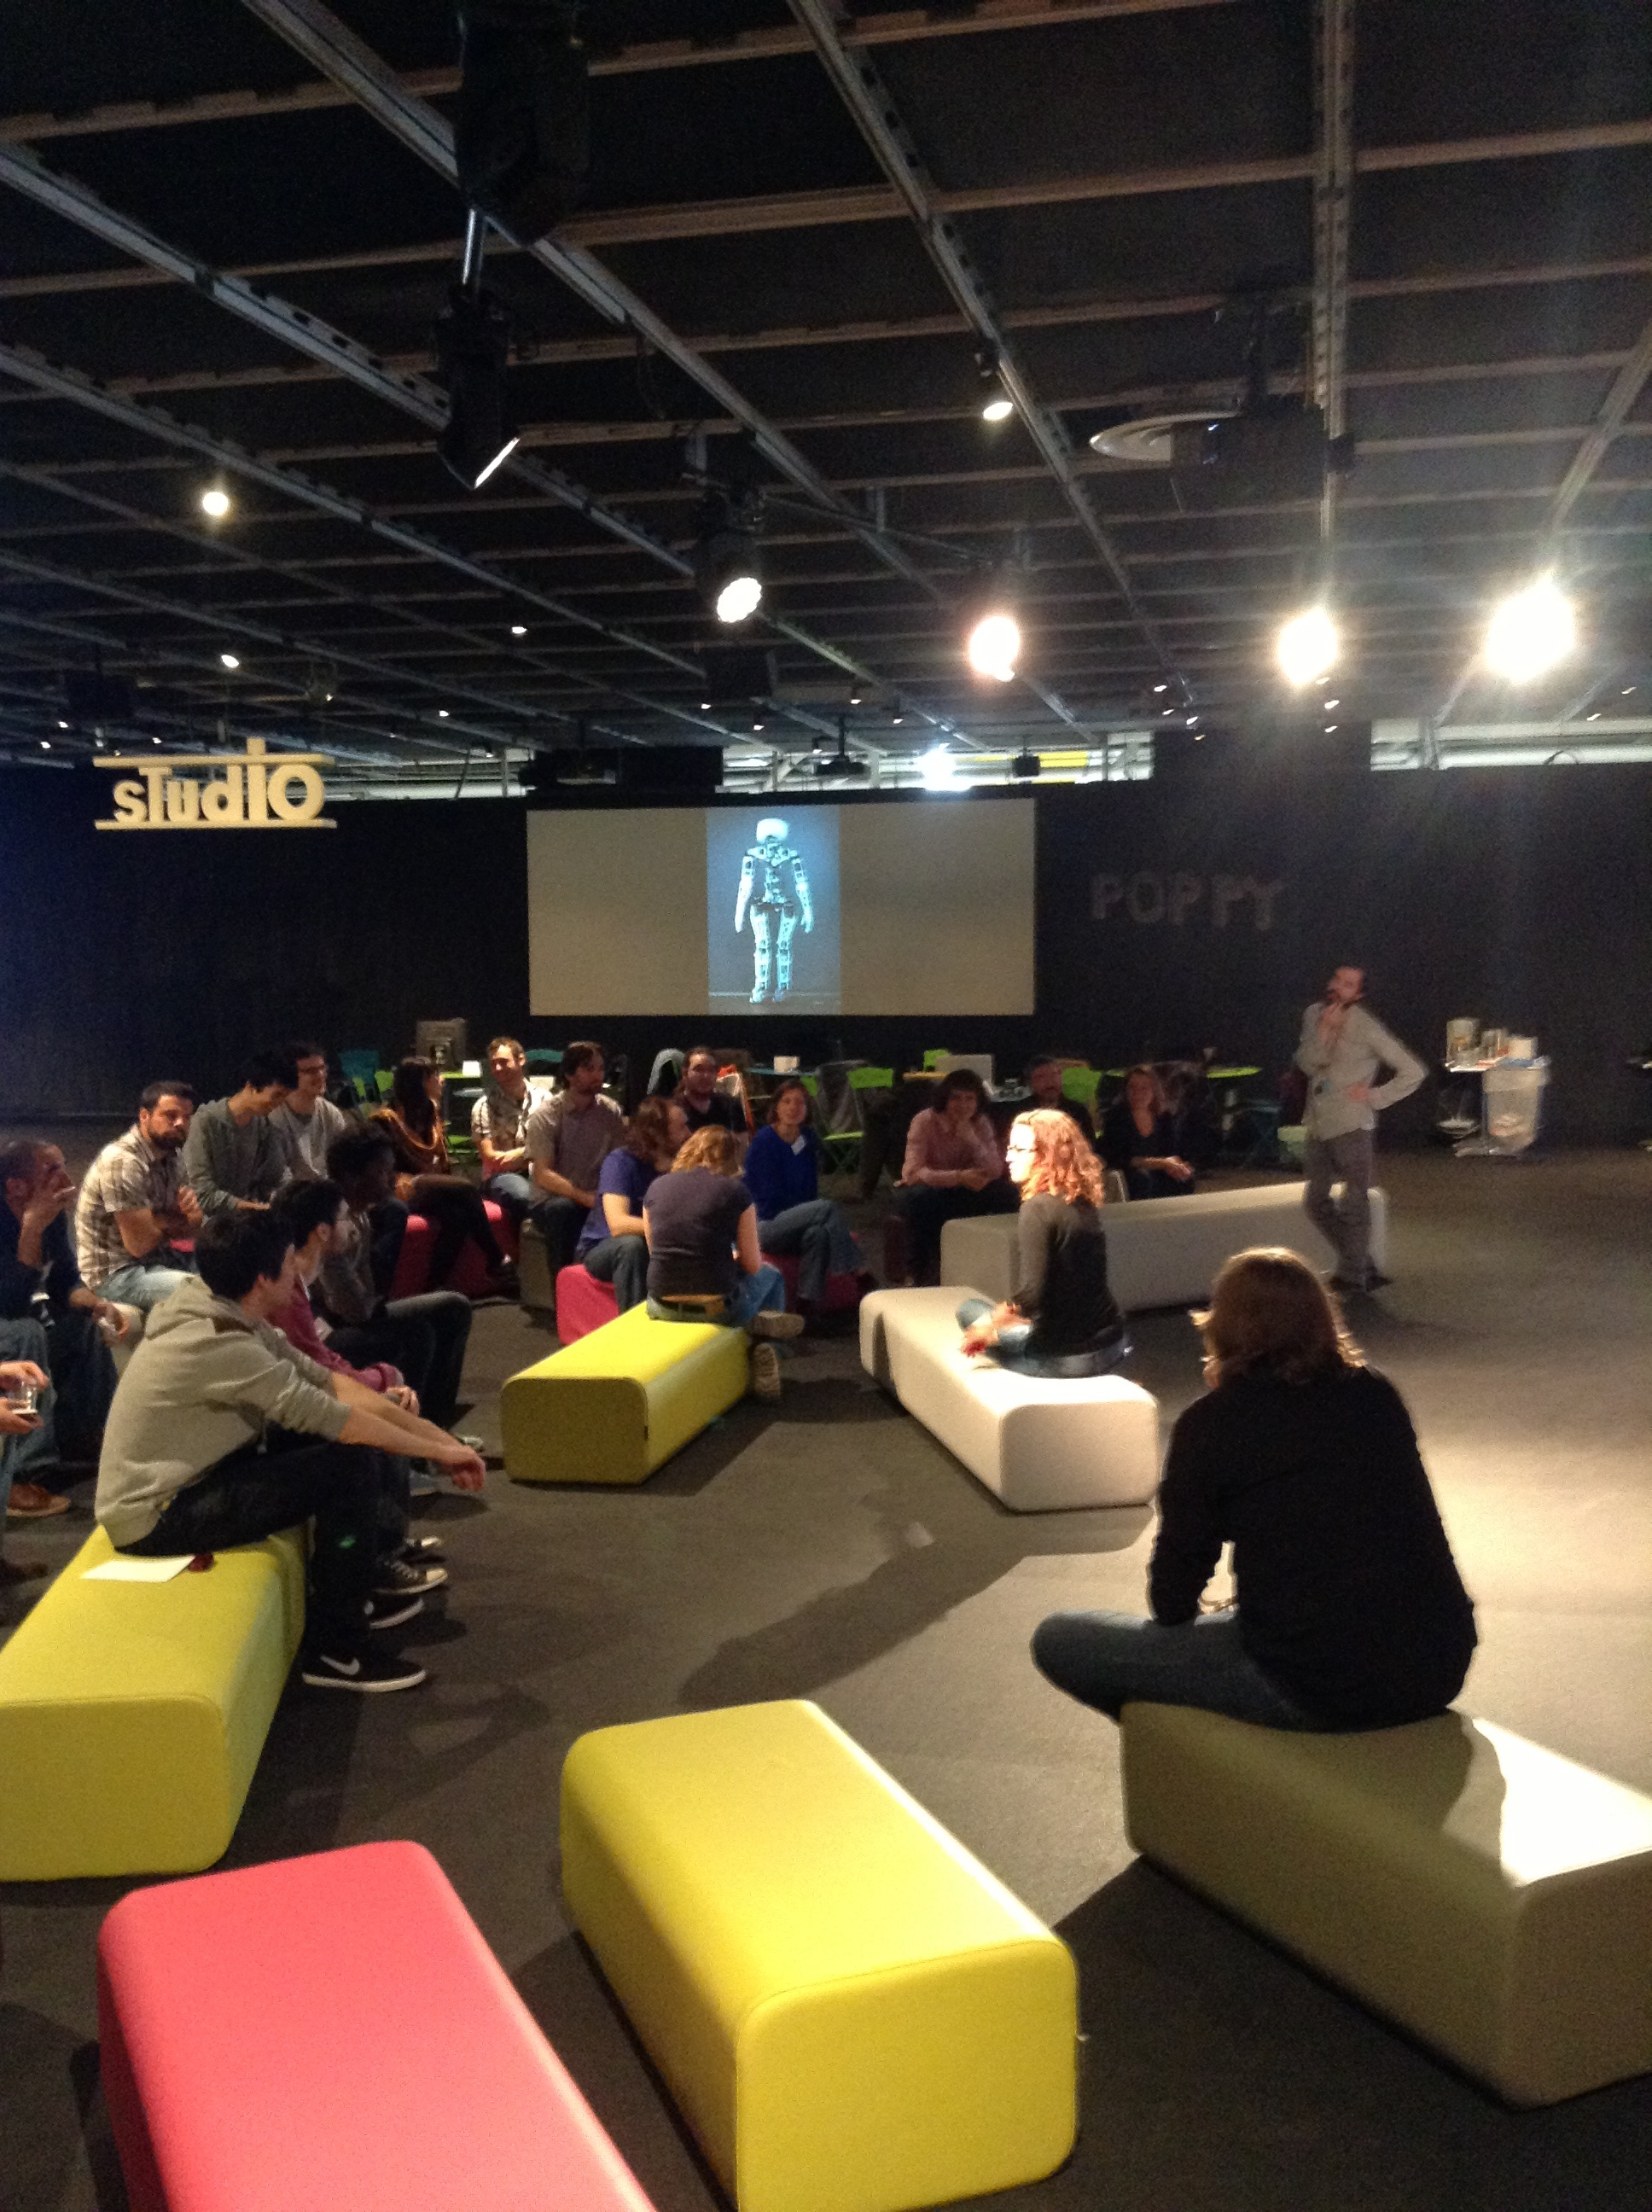
\includegraphics[height=5cm]{hackathon_intro.jpg}}
    \hfil
    \subfloat[][Poppy's hackathon]{\includegraphics[height=5cm]{hackathon_setup.jpg}}
    \caption{}
    \label{fig:universience_hackathon_orga}
\end{figure}

Participants were dispatched around several workshops during the two days. While a group was dedicated to the actual assembly of the different Poppy parts, others were exploring how to program the robot in Python or working on designing and 3D printing hardware improvements.
During the weekend, near to 100 visitors came to visit the workshop and some of them integrate the hackathon.

In two days, this group of new users, self-trained using only online documentation has been able to build from scratch the whole robot and make it move using the Pypot library. Eventually, two young students got an idea: 3D printing an ankle that could give some articulated movement to Poppy's feet. They designed a new original semi-passive solution for the ankle joint as well as a robot helmet which was 3D printed and assembled within the time of the workshop.

\begin{figure}[]
\centering
    \subfloat[][]{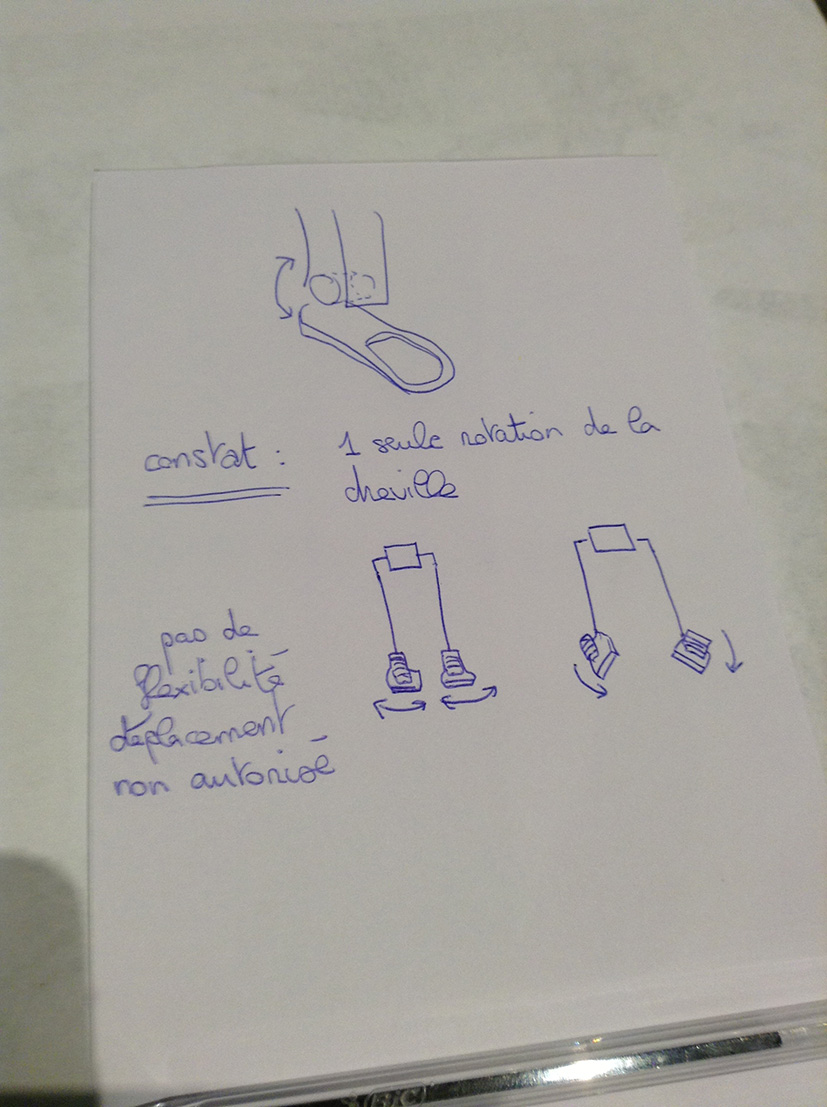
\includegraphics[height=5cm]{hackathon_conception1.jpg}}
    \hfil
    \subfloat[][]{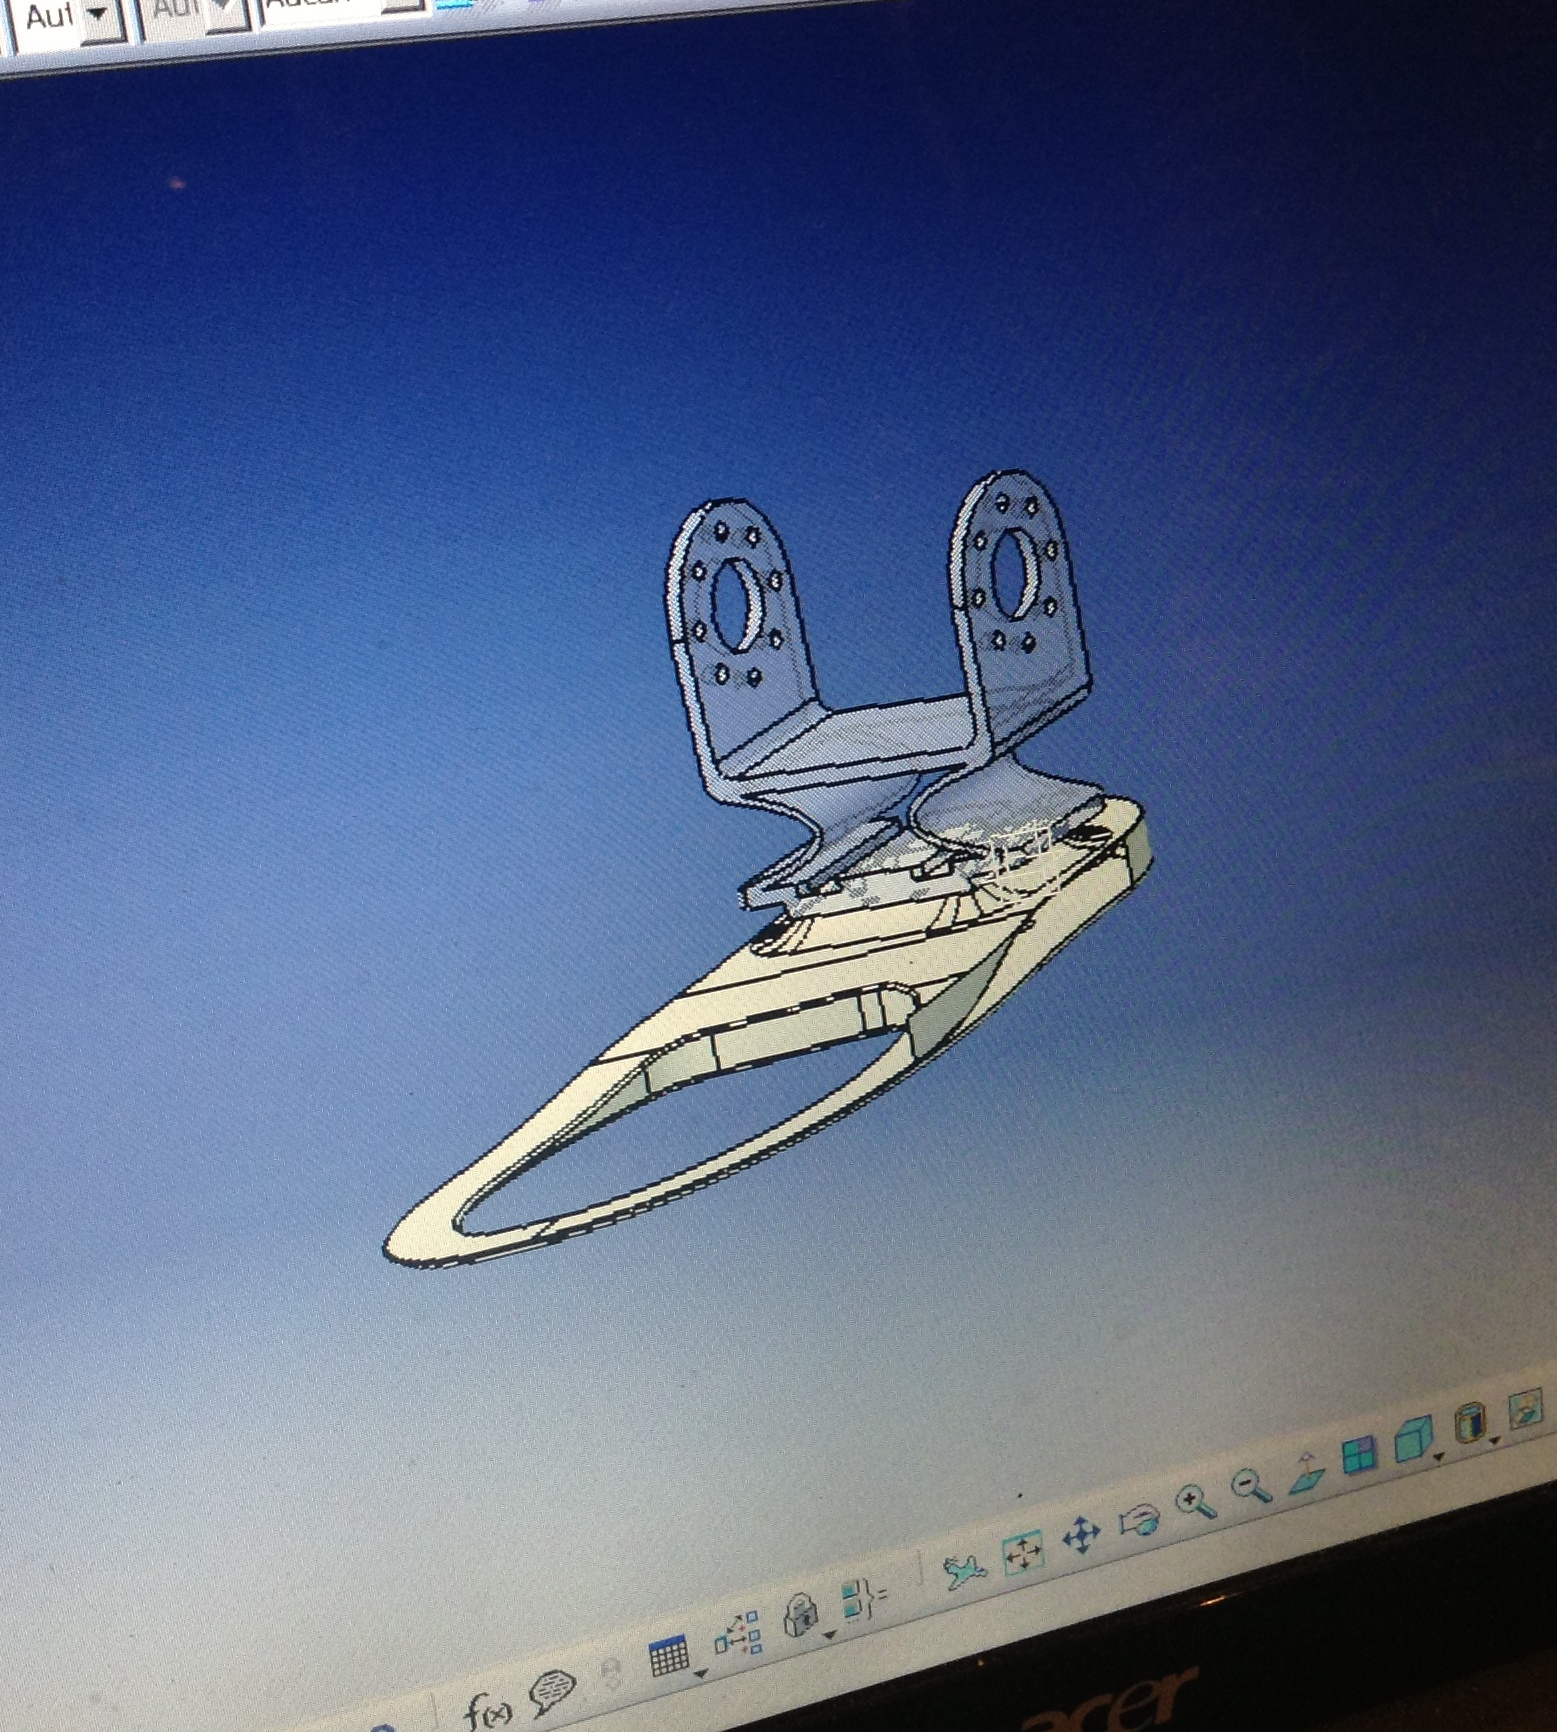
\includegraphics[height=5cm]{hackathon_conception2.jpg}}
    \hfil
    \subfloat[][]{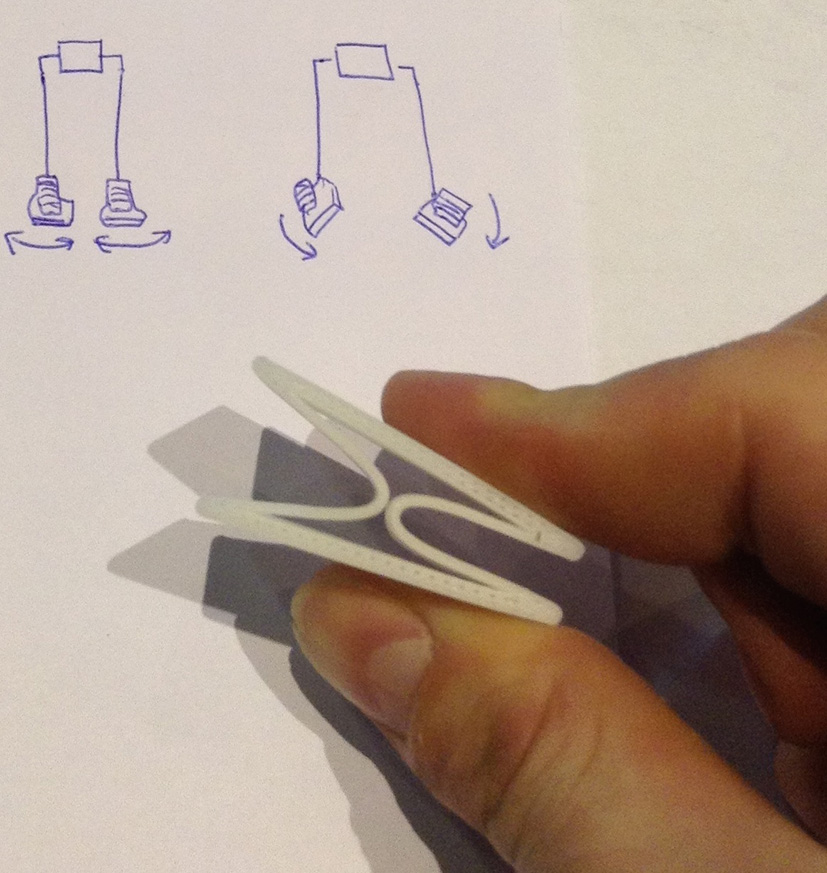
\includegraphics[height=5cm]{hackathon_conception3.jpg}}
    \caption{}
    \label{fig:universience_conception}
\end{figure}

This experiment did not only show that the platform was easily usable in an educational context with users of all ages, and was reproducible in two days by a little group, but it also showed high educational value as testified by users and educators (see \url{https://forum.poppy-project.org/t/poppy-project-at-la-cite-des-sciences-et-de-lindustrie/}).

\begin{figure}[h]
\centering
    \subfloat[][]{\includegraphics[height=4.5cm]{hackathon_assembly1.jpg}}
    \hfil
    \subfloat[][]{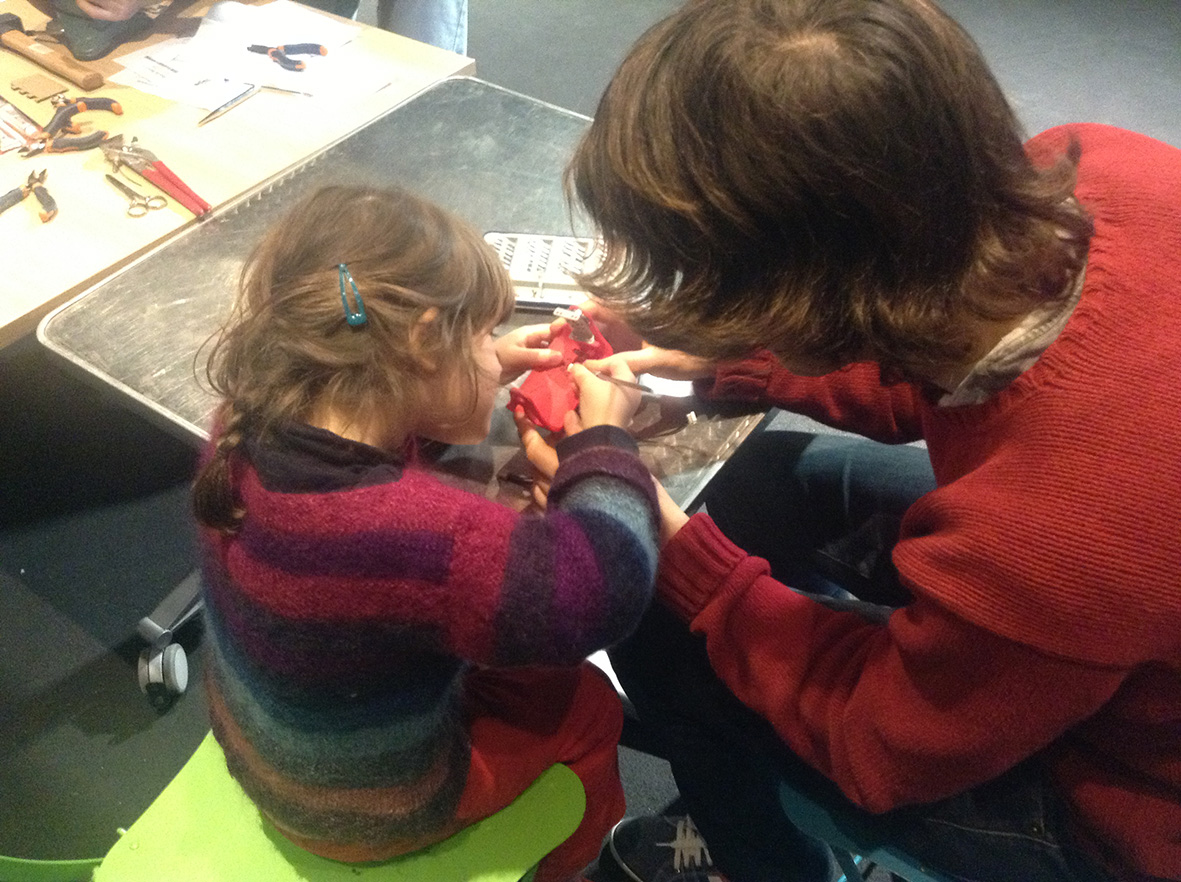
\includegraphics[height=4.5cm]{hackathon_assembly2.jpg}}\newline
    \subfloat[][]{\includegraphics[height=4.8cm]{hackathon_assembly3.jpg}}
    \hfil
    \subfloat[][]{\includegraphics[height=4.8cm]{hackathon_last_screw.jpg}}
    \caption{}
    \label{fig:universience_assembly}
\end{figure}

Indeed, because Poppy is not a "black box". It has to be assembled and even if it is quite simple to be programmed, people needs to understand the basic of programming and then explore by trial-error the way to achieve a desired behaviour. Thus using Poppy leads to the use of the scientific synthetic methodology "understanding by building" and constructivist learning approach which are great methods to both foster critical thinking and create deep reflexions on the understanding of nature. People are then more open and receptive, allowing the mediation team to get their message in an effective way and maybe push further scientific analysis with the public.

\begin{figure}[h]
\centering
    \subfloat[][]{\includegraphics[height=5cm]{hackathon_poppy_assembled.jpg}}
    \hfil
    \subfloat[][]{\includegraphics[height=5cm]{hackathon_first_trial.jpg}}
    \caption{}
    \label{fig:universience_conception}
\end{figure}


Since this hackathon, Poppy is used by the Universciences Fablab but also for activities and animation aside the "Robotic Art" exhibition (08/04/2014 to 04/01/2015) \figurename~\ref{fig:universcience_art}. It took part to the opening of the exhibition on April the 8th, and is part of the science show "l'ère des Robots" (The robots era) see \url{http://www.cite-sciences.fr/fr/au-programme/expos-temporaires/art-robotique/activites-associees/}.

\begin{figure}[]
\centering
    \subfloat[][]{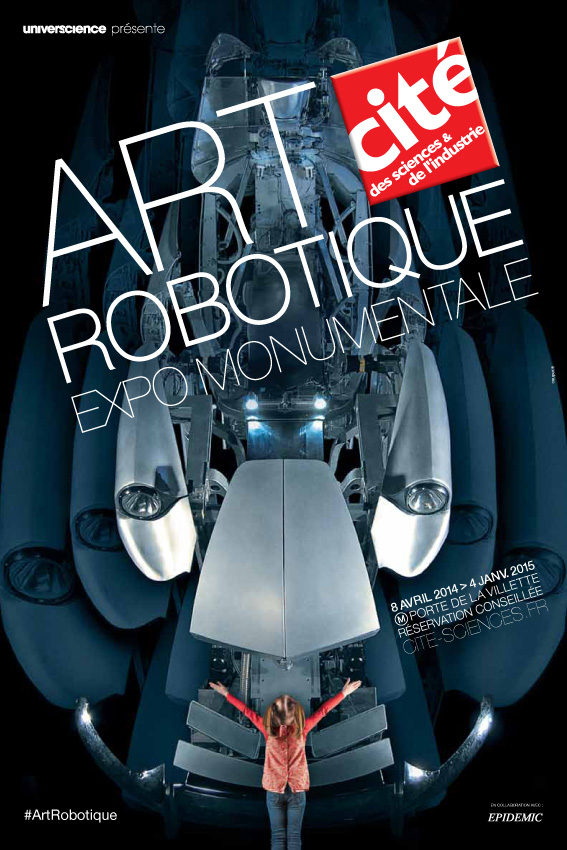
\includegraphics[height=6cm]{art-robotique_universcience.jpg}}
    \hfil
    \subfloat[][]{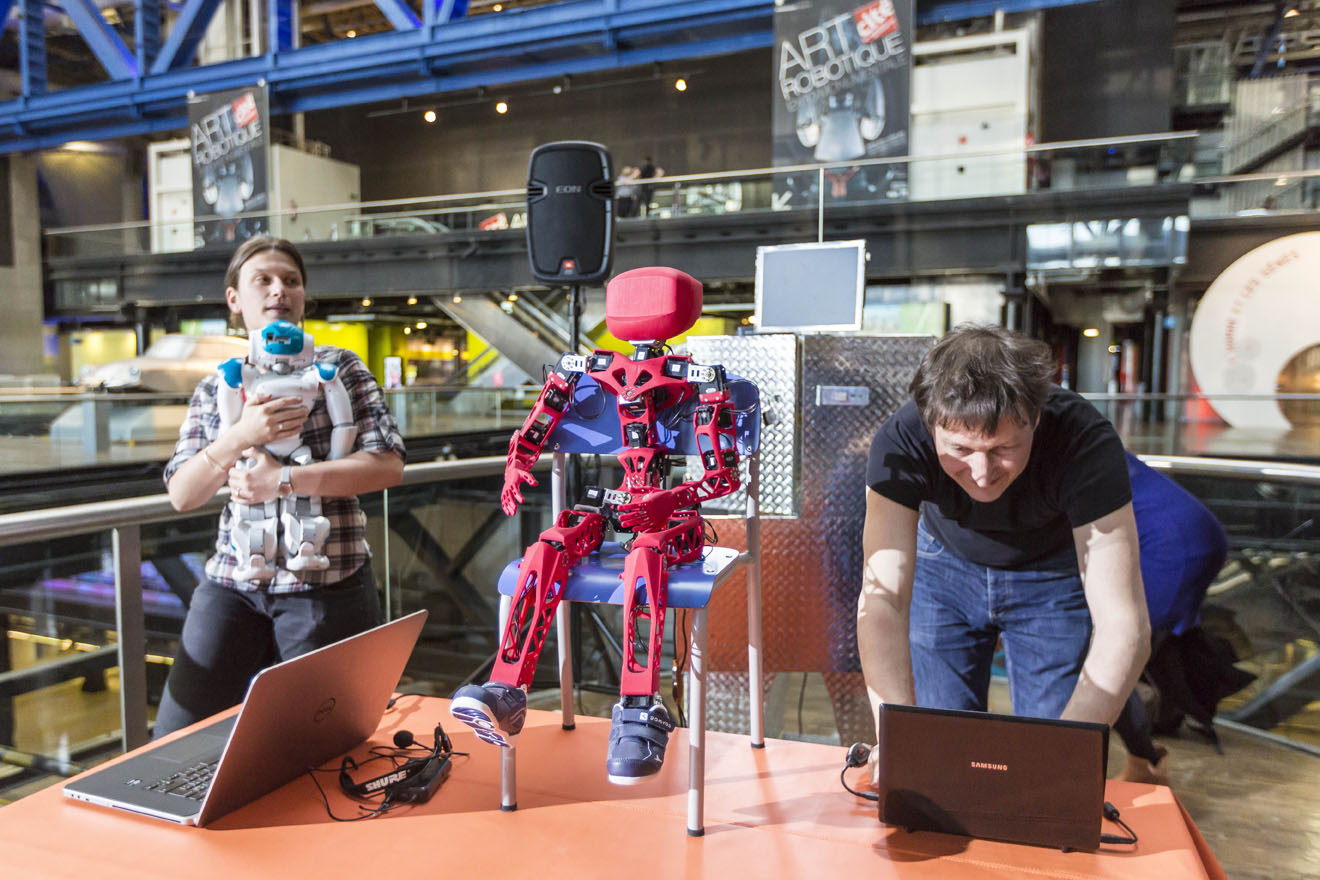
\includegraphics[height=6cm]{poppy_demo_universcience.jpg}}
    \caption{}
    \label{fig:universcience_art}
\end{figure}


\newpage
\section{Engineering School}

Two students cognitician working on a TER were interested by the design of emotion and studying the reaction of


I were really busy and did not have time to take care of their project, I just give them Poppy and spent 10-15 min explaining how to use it.



This research was conducted jointly by two students from the UFR Sciences et Modélisation of the University of Bordeaux with the cooperation of the INRIA FLOWERS team.

This study aims to better understand human-machine relations and how they fit into our society.


\newpage
\section{High school project} % (fold)

After the artistic residency which happened in the Saintonge Sainte Famille high school's chapel (see chapter~\ref{cha:art}), some teachers have been interested by the educational potential of the Poppy project and wanted to integrate it as a common thread along the school year.

Poppy has been first thought for research purposes and seems to be well adapted for higher education training. Thus using Poppy in the secondary education seems overkill as it is expensive and the use of high quality servo-actuators is not really justified. However the experience with high-school students is still interesting and we accepted to take this opportunity to make a pilot experiment.


The experiment took place in the Saintonge Sainte Famille high school on May the 26th \& 27th. The organisation was made around several working groups during three 4-hours sessions. The last two hours were dedicated to PowerPoint presentations in the lecture hall to share with other students what they did (see \figurename~\ref{fig:saintonge_support} and \figurename~\ref{fig:saintonge_demonstration})

The experiment concerned near 40~\emph{première STI2D} students (UK equivalent to Year 12) preparing a professional baccalaureate and three teachers from TODO, TODO and TODO specialities.

\textbf{For the teachers}, the main goal was to get experience of using such tool in a project context and evaluate the promises and limit for their educational mission.

\textbf{For us}, we were interested by the reaction of young students to Poppy and get an opinion on the relevance of Poppy for education at this level. Also, it was a real crash test of our conception (hardware and software) in non-experimented hands.

For this first pilot experiment, we decided to reduce the cost by using only a sub-part of the whole Poppy. For me the most relevant part for high-school students was the upper body (thorax, head and the two arms), because it avoids to work on complex sensory-motor behaviours such as balancing and walking while keeping the expressivity potential of Poppy. The total cost to get Robotis Dynamixel motors, electronics and 3D printing service was 2500\texteuro (20 \% tax included).

\textbf{TODO: Figure with the upper body of Poppy and the BOM list}

Like the Universcience hackathon (see section~\ref{sec:poppy_universience}), students were dispatched on several sub-tasks we will describe in the following sections.


\subsection{The Poppy's assembly} % (fold)

The assembly of Poppy was divided in three groups: one was doing the assembly of the thorax and the head (4 motors) and two other ones for each arm (3 motors). At the end of the first day the half-Poppy was assembled (see \figurename~\ref{fig:saintonge_assembly}) with quite few troubles.

\begin{figure}[h!]
\centering
    \subfloat[][Motor assembly and configuration]{\includegraphics[height=4.4cm]{saintonge_assembly1.jpg}}
    \hfil
    \subfloat[][Thorax assembly]{\includegraphics[height=4.4cm]{saintonge_assembly2.jpg}}
    \hfil
    \subfloat[][Arm assembly]{\includegraphics[height=4.4cm]{saintonge_assembly3.jpg}}
    \hfil
    \subfloat[][Poppy almost finished, only the face is missing]{\includegraphics[height=4.4cm]{saintonge_assembly4.jpg}}
    \caption{Poppy was assembled by 3 parallel working groups divided into thorax+head and the 2 arms. At the end of the first day, the half-Poppy was assembled and functional. }
    \label{fig:saintonge_assembly}
\end{figure}

However, as I will discuss with more detail in the further section REF, we experienced some difficulties with high school Internet connection and all documentation is online\dots So it was unfortunately a bit difficult to evaluate if our documentation was clear enough for high-schools student. Yet, from that I experienced explaining the "how-to", it appears we need a highly detailed documentation for the very first steps. Then general guidelines seem to be enough to achieve a well-assembled Poppy robot.

\subsection{Python programming with pypot}

Two working groups were dedicated to learning basic Python programming with pypot (see \figurename~\ref{fig:saintonge_software}). The teacher has selected these students because of their enthusiasm for computer science. Indeed when they heard about the Poppy project few weeks ago, they got interested by Python and began to look for further information on Internet.

The first hours of the software workshop have been complicated. The school computers were not out-dated but were under windows and used by a lot of different people, so configurations were not consistent between machines and sometimes a bit exotic. The installation of the necessary tools (Python + packages + text editor) has been really long and painful. I will come back to this point in the section REF.

Once desktop were setup, students took a look to the basic pypot tutorials\footnote{\url{http://poppy-project.github.io/pypot/tutorial.html}}. They first tried to control one Dynamixel motor (reading/setting positions). Then they use a group of motors (each having one Poppy arm) and we introduce the pypot robot configuration file. At this point they were able thanks to the basic pypot tutorial to create a robot with specific motor configuration and make it move by setting direct goal positions or using sinus trajectories. This improvised complexity slope leads them to a well understanding of the very basic features of pypot and Dynamixel motor properties in just 2 hours and without any previous Python experience.

Then the hardware groups get Poppy assembly done, the software group modified the Poppy's configuration file and adapted it to their own Poppy. At the end of the first day, the two groups were able to make their Poppy move.

The software guys continued their work the next day, trying to create more complex behaviours. One of them (see \figurename~\ref{fig:saintonge_motivated_software_guy}), managed to create on his own (I did not write any line of code) the copy-arm behaviour we showed in the Poppy overview video\footnote{http://vimeo.com/poppyproject/poppyoverview}. Then he explained how he did it to his classmates (see \figurename~\ref{fig:saintonge_knowledge_transmission}).

After learning how this behaviour was done, another group decided to make Poppy clap its hands. By trial-error they manage to make the basic motion using sinus. These self-exploration raises the need to understand what is a variable, how a sinus acts and they experimented by their own the different sinus properties such as frequency, amplitude and even offset. As Mitchel Resnick explained in~\cite{resnick2009scratch}, here the meaningful context of making a robot move leads students to be curious about mathematics and computer science concepts.


\begin{figure}[]
\centering
    \subfloat[][One software working group discussing pypot with their teacher]{\includegraphics[height=4.4cm]{saintonge_soft1.jpg}}
    \hfil
    \subfloat[][The two software groups discussing about Poppy's configuration file]{\includegraphics[height=4.4cm]{saintonge_soft2.jpg}}
    \hfil
    \subfloat[][Experimentation trough trial-error]{\label{fig:saintonge_motivated_software_guy}\includegraphics[height=4.4cm]{saintonge_soft3.jpg}}
    \hfil
    \subfloat[][Transmission of knowledge between classmates]{\label{fig:saintonge_knowledge_transmission}\includegraphics[height=4.4cm]{saintonge_soft4.jpg}}
    \caption{High-school students discovering programming with Python and the pypot library}
    \label{fig:saintonge_software}
\end{figure}

\subsection{Design of a Poppy's support in Solidworks} % (fold)

As we were only building the very upper part of the robot, several students worked in pair to design wheeled platform supporting their own Poppy version. The teacher instructions were to create a mobile support for their Poppy with enough room to include batteries and a computer.

For most of them it was the first introduction with the use of parametric modelling tools. However, the final result (see \figurename~\ref{fig:saintonge_support}) is quite impressive. All working pair managed to finish the design of the basic idea of their conception choice and integrate the Poppy robot.

A really interesting point is the fact they all choose a different conception to make their support move. Some used caterpillar, others four wheel or two and a free wheel. The Poppy robot gives a pretext to creation and let students free to explore. However

\begin{figure}[]
\centering
    \subfloat[][Caterpillar design]{\includegraphics[height=4.5cm]{saintonge_support1.jpg}}
    \hfil
    \subfloat[][Four independent wheel design]{\includegraphics[height=4.5cm]{saintonge_support2.jpg}}
    \hfil
    \subfloat[][Two motorized and a free wheel]{\includegraphics[height=4.5cm]{saintonge_support3.jpg}}
    \caption{Students of the design support work group explain their choices to others.}
    \label{fig:saintonge_support}
\end{figure}


\subsection{Documentation } % (fold)

Finally, the other students were in working groups in charge to report the different workshops activities. They had to take picture of the robot assembly and get a global view of the project to extract meaningful information for building SYSML diagrams with MagicDraw. They had also to train English and report translation of technical words in a robotic context.

The students of these groups were way less enthusiasts than other, some even discreetly sneaked into other workshops. Of course, building and programming a robot is way more fun than reporting it. This shows some limitation of project such as Poppy, there is no enough work for lot of students, which introduces content interest inequalities.

% \begin{figure}[]
%     \begin{center}
%         \includegraphics[width=0.8\linewidth]{saintonge_poppy_first_moves.jpg}
%     \end{center}
%     \caption{Caption here}
%     \label{fig:saintonge_result}
% \end{figure}

\begin{figure}[]
\centering
    \subfloat[][]{\includegraphics[height=4.3cm]{saintonge_poppy_first_moves.jpg}}
    \hfil
    \subfloat[][]{\includegraphics[height=4.3cm]{saintonge_demo1.jpg}}
    \caption{After finishing the hardware assembly, students began to make Poppy move using the pypot library. They mannasge in just few hours to create impressive movement and behavior while never having developed using PythoN.}
    \label{fig:saintonge_demonstration}
\end{figure}



\section{Lessons learn} % (fold)

These two experiments were really instructive as we got the chance to have real crash-test in ecological conditions: a group of people left alone to build a complex robot in a Fablab style environment and real students in their high school and with their own equipment. As I personally took part of the workshop in the high school, this section resuming the educational interests will be more oriented toward this last experiment.

For example, in ~\cite{resnick2008sowing}, Mitchel Resnick quote the experience a teacher had while using Scratch for a school project:
\begin{quotation}
    There is a buzz in the room when the kids get going on Scratch projects. Students set design goals for their projects and problem-solve to fix program bugs. They collaborate, cooperate, and co-teach. They appreciate the power that Scratch gives them to create their own versions of games and animations.

    \signed{Karen Randall, teacher at the Expo Elementary School in~\cite{resnick2008sowing}}
\end{quotation}

This description is actually pretty close from that I experienced with the high school students. I was really surprised and pleased how the students were able to switch from a pyramidal way to learn, where they are passive and expect the teacher to transmit some knowledge, to a flat one or even a bottom-up one, where students are pro-active and ask the teacher for explanations, use them to understand novel concept then transmit to their classmates.

This experiment turns out to be much more instructive than expected and lead to the learn of several lessons:

\textbf{1- A robotic project is very motivating:} the goal of having their own "cool" robot moving was a really impressive motivation fuel. Students were not discouraged by the difficulties raised on the path to achieve their goal. Also they had a positive way to try to overcome them. Surprisingly, they did not seem bored by all the inconveniences that occurred such as installing tools on machine, Python syntax tricks or redo the mounting of an assembly because they made a small mistake. Actually, the teacher seemed way more annoyed than his students.

\textbf{2- Robots provide a meaningful context, conductive to the learn of mathematical and computer science concepts:}

I cannot relate for other country but in France, the way we learn math in junior and high school is totally meaningless. We learn to do calculus just because the mathematical program says we have to. In this context math looks like an intellectual game without any daily life application\dots

However problems raised when making and controlling a robot require the use of math and students see in them the tools needed to reach their goal. They are learning math because it is on the way to achieve a cooler and more rewarding goal. In this pilot experiment, the students were from a professional baccalaureate, typically the kind of students saying they are not "a born mathematician" and so will never succeed in doing it. However, while trying to control Poppy, especially to make it applause, they were confronted to mathematical problems and used sinusoidal signal to achieve it. Using Poppy they were able to see, immediately and in the real life, the usefulness of sinus and eventually began to explore by their own the role of each parameter (amplitude, frequency, phase, offset).

The same effect can be observed in teaching computer science and programming. Indeed, having to deal with weird syntax rules, complex commands and austere interfaces are discouraging. Using robot make the programming experience way different. You are not studying computer science to print characters on a black system console, but you are using programming to make a robot move!
During the experience with the high school students I saw two main advantages. First, the motivation of making a robot move helps students to overcome the syntax tricks problems. Second, teaching Object-oriented programming (OOP) using actual object is way easier. Indeed, understanding that a motor is an object with properties and functions is really meaningful.


\textbf{3- Poppy is open source, it can be hacked and adapted to the needs:}
The fact Poppy is at the same time open source, 3D printed and cool is definitely a killer application for education. Its design catch the students attention while the free use of all its sources allow teacher to create educational content based on exploring and understanding the state of the art and let students express their creativity by hacking the platform.


Also, because Poppy is modular, it allows teachers to adapt its use to theirs needs. Here, it was possible to only take one part of the robot and use the student’s creativity to create the missing elements. This kind of usage will not be possible if Poppy was a commercially and closed robot.

\textbf{4- Do not rely on educational equipment:}
Internet access was really bad, so slow our forum could not be displayed. Also even if school computers are quite up-to-date, there are used by a lot of different and more or less expert users and have potentially incompatibilities or weird configuration. So we cannot expect to find a working environment close to the one we have in our labs.
We have either to ensure before the workshop that every desktop is ready or use tools more robust to system configuration issues.

\textbf{5- Well-designed and stand-alone IDE is needed.}

The previous point showed us that the current way to work with Poppy was not adapted to its use in high school. Indeed, we lost almost all the first 4-hours session just trying to set-up a development environment allowing the use of the pypot library. We eventually gave-up on certain high-school machines and we stopped when we got the minimum required tools. However there are complementary tools such as ipython notebook that greatly improves the convenience when programming in Python.

Thus eventually, high-school students managed to develop complex behaviour with Poppy but the teacher for their enthusiasm about computer science selected them. Probably students without prior excitation would give up facing so much system setup difficulties.

This problem conducts us to look for improvement and we eventually found an interesting way to overcome this setup issues. The week after, we submit a project to the Aquitaine Region call about the design of a development environment adapted to the use of Poppy in educational context. We will describe more about this project in the future work (see REF).


\textbf{7- Content should be translated in the native language:}

The Poppy project was initially a research project and English is the only language used for information and documentation. Yet this choice is a real problem in the educational world. In France, a large amount of people is not fluent or not at all able to speak and understand English. Of course, within the students, the younger they are the less they are confortable with foreign languages. In addition, the teacher English level is also pretty bad and so the fact information we give is in English is a stumbling block to the diffusion of Poppy in the French educational system.



\section{Discussion} % (fold)

Open source 3D printed robotic can help in the creation of meaningful contexts allowing people and students to explore several scientific aspect among them, computer science, mechanics and electronics. In particular, the use of Poppy can be a great gamification tool for scientific mediation and educational purpose.

Because it allows people to explore by themselves some basics of robotics, Poppy confront users to the use of programming and mathematical concept which can arouse the general public to complex scientific challenges and the usefulness of such technical sciences often studied in a meaningless context.

Also during a small amount of time, students are scientific researchers lost in an open field of exploration. It is a really great way to introduce people with the scientific thought, doing experiments by trial-error, trying to understand how to achieve a desired goal, creating model using math or algorithms.

However, even if the two experiments conducted showed a high potential about Poppy societal impact for education, there are still several limitations:

First, Poppy is low cost for a research labs but it is too expensive to have an actual impact in the educational system. Its current cost makes it accessible only in some privileged high schools. Also, even in the high schools, which can afford such robot, it is only possible to have one or two which leads to inequalities in the project course. Few students get the chance to build the robot or make it move while other are passive and cannot take part to the activity.

However, using such high quality actuators is not really relevant for educational uses, at least before baccalaureate. While the humanoid shape seems to really have an impact on the students’ motivation, the fact Poppy is tall and compliant is not a real need. We could and should definitely propose a cheaper alternative more adapted to schools and high schools. Poppy being still relevant in universities, engineering schools and of course research labs.

Second, the way to control the robot is not adapted in educational context. Having to spend time on installing each needed packages and then figure out why the system crashes is not really interesting or relevant for students. They should rather spend time on programming and using the robot. Also, ones can notice successful educational project such as Arduino~\cite{banzi2009getting} and Thymio~\cite{shin2014visual}  propose such plug'n'play IDE (see \figurename~\ref{fig:eductationnal IDE}).

\begin{figure}[]
\centering
    \subfloat[][Arduino]{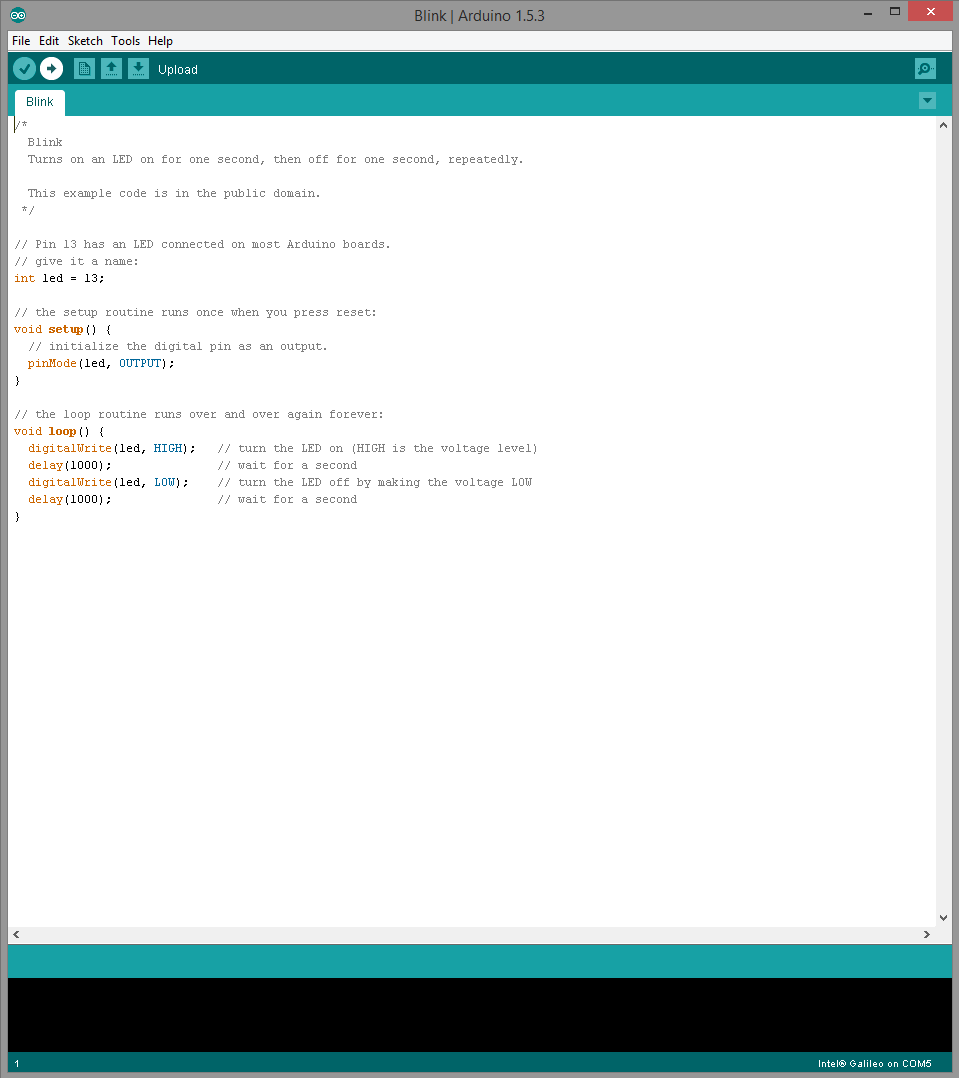
\includegraphics[height=6cm]{arduino_IDE.png}}
    \hfil
    \subfloat[][Thymio 2 IDE]{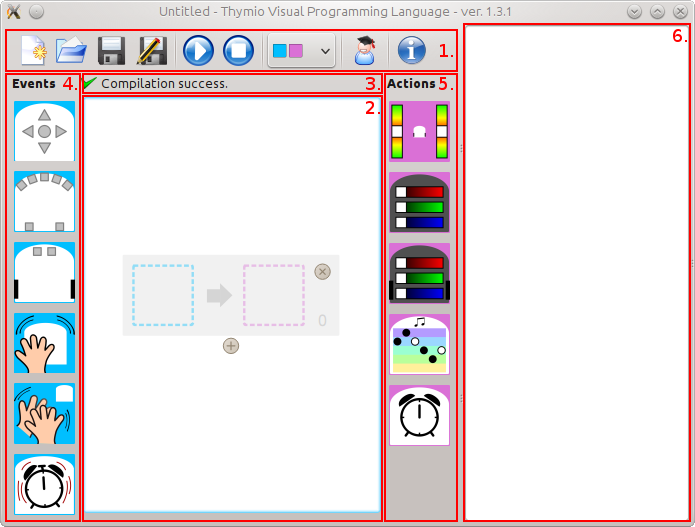
\includegraphics[height=6cm]{thymio_IDE.png}}
    \caption{Arduino and Thymio are stand-alone IDE allowing to have plug'n'play device, immediately useable right out the box. Also, the user interface is done to make the code readaction easy to write and debug. Creating great IDE seems essential toward the success in the educationnal field.}
    \label{fig:eductationnal IDE}
\end{figure}


Finally, we should be careful that the activities associated with Poppy are not only playful but have a real educational impact. To do so, actual teachers need to create educational content. Of course it is easy to get the students attention for 2 days with project as fun and playful as Poppy but creating relevant content running as projects along a whole school year is way more challenging.

Confronted to these three points, we found promising technical solutions and we set up partnership with educational local actors to propose a project to the Aquitaine Region in order to get the resources needed for the development


\section{Future work} % (fold)

As we explained previously, experiments involving Poppy have shown potential for educational application. However, the cost of Poppy, the complex setup to run pypot and the lack of educational content, the relevance of Poppy in high schools and first years of universities is still questionable.

So we decided to adress the needs and we launched a parternship with a famous engeeniring school (ENSAM) and a high school (Saintonge Sainte Famille) towards the creation of educationnal content and users experimentation in actual context.

The Poppy Education project aims to realize, exploit and disseminate a teaching platform based on the use of Poppy for integrated learning of computer sciences and engineering. Especially it aims to provide:
\begin{itemize}
    \item An open source integrated development environment (IDE) based on web technologies with an embedded Python interpreter. This application can be stand-alone and will allow both the sharing and deployment of educational resources around the use of the robot, and a friendly interface to program and monitor it.
    \item A mini version of the current Poppy robot. Using \$20 Robotis Dynamixel XL320, it would be possible to achieve the building of a 30cm tall 3D printed Poppy for around \$500.
    \item Educational content using this environment, Poppy and Poppy mini in real situations with high school and bachelor curses (thanks to our partnership with ENSAM and Aerocampus).
    \item The dissemination of these educational tools under open source and Creative Commons licenses.
    \item The translation of the software, the documentation and educational content in French and English. Other language translation will be done with external contributions.
\end{itemize}




% \subsection{MOOC} % (fold)
% Papert in ~\cite{guzdial2004programming} argued that programming languages should have a low floor (easy to get started with) and a high ceiling (opportunities for increasingly complex projects over time). In addition, we believe that languages need wide walls (supporting many different types of projects, so that people with different interests and learning styles can all become engaged). Satisfying the triplet of low-floor/high-ceiling/wide-walls hasn’t been easy.

% Mooc' critics are mostly "constructionists". The school of thought holds that kids lose interest in math beacause it's so often taught as a bunch of mechanical routines you follow to solve problems disconnected from the every day life.

% Constructionists argue that it's better to give kids activitiies that let them discover the principles of math and physics on their own-for instance, having them play around with kid-friendly programming languages like Logo. "Students 'fumbling around' is actually where the learning happens"

% Another limitation of khan's site is that the drilling software can ahadle only sibjects where the answaers are unambiguously right or worng, like math or chemistry.

% If khan is truly liberating students to advance at their own pace, it's not clear that the schools will be able to cope. What happens when, using khan acamdemy, you wind up with kid in fifth grade who has mastered high school trigonometry and physics but is still functionning like a regular 10-year-old when it comes to writing, history and social studies ?

% subsection mooc (end)


% Mooc' critics are mostly "constructionists". The school of thought holds that kids lose interest in math beacause it's so often taught as a bunch of mechanical routines you follow to solve problems disconnected from the every day life.

% Constructionists argue that it's better to give kids activitiies that let them discover the principles of math and physics on their own-for instance, having them play around with kid-friendly programming languages like Logo. "Students 'fumbling around' is actually where the learning happens"

% Another limitation of khan's site is that the drilling software can ahadle only sibjects where the answaers are unambiguously right or worng, like math or chemistry.

% If khan is truly liberating students to advance at their own pace, it's not clear that the schools will be able to cope. What happens when, using khan acamdemy, you wind up with kid in fifth grade who has mastered high school trigonometry and physics but is still functionning like a regular 10-year-old when it comes to writing, history and social studies ?




